% pdflatex -shell-escape template_rapport.tex

\documentclass[a4paper,oneside]{article}

\usepackage[frenchb]{babel}
\usepackage[utf8]{inputenc}
%\usepackage[T1]{fontenc}
\usepackage{graphicx}
\usepackage{amssymb} 
\usepackage{amsmath}
\usepackage{hyperref}
\usepackage{fullpage}
\usepackage{titlesec}
\usepackage{fancyhdr}
\usepackage{nopageno}

%%%%%%%%%%%%%%%%%%%%%%%%%

\title{Rapport du projet Bataille Navale (IA)}
\author{Tholliez Alexandre}
\date{14 juin 2017}

\makeatletter
\pagestyle{fancy}
\fancyhf{}
\fancyhead[L]{}
\fancyhead[C]{}
\fancyhead[R]{}
\renewcommand{\headrulewidth}{0pt}
\fancyfoot[L]{\@title}
\fancyfoot[C]{}
\fancyfoot[R]{page \thepage / \pageref{myLastPage}}
\renewcommand{\footrulewidth}{0.4pt}

%%%%%%%%%%%%%%%%%%%%%%%%%

\begin{document}

%%%%%%%%%%%%%%%%%%%%%%%%%

\thispagestyle{empty}

\Large
ULCO - L3 Informatique

\vfill 

\Huge
\begin{center}
\@title
\end{center}

\normalsize

\vfill 

\paragraph{Étudiants : Quentin Coloos - Alexandre Tholliez - Thomas Prunier - Benoît Verhaghe }

\paragraph{Encadrant : Ahmad Mazyad}

\paragraph{Date de début : 29 mai 2017 }

\paragraph{Date de fin : 16 juin 2017 }

\paragraph{Objet du projet : Création d'un jeux vidéo avec une Intelligence Artificielle }

~

\vfill 

\noindent\rule{\linewidth}{0.5pt}

\tableofcontents

~\\
\noindent\rule{\linewidth}{0.5pt}

\clearpage

%%%%%%%%%%%%%%%%%%%%%%%%%

\section{Présentation du projet}


\subsection{Analyse de la demande}

\subsection{Contexte}

Dans le cadre du projet de fin de Licence, il nous était demandé de choisir entre :

  - Le développement d'un jeu vidéo en réseau en C++

  - Le développement d'un anti-spammer.

  - Le développement d'un jeu vidéo avec une Intelligence Artificielle avec langage de programmation au choix.

Dans ces 3 projets, seul l'anti-spammer ne nous intéressait pas du tout.
Nous devions donc choisir entre l'IA ou le réseau, n'ayant aucune connaissance en réseau nous avons décidé de nous orienter vers le projet avec une IA.

Le langage de programmation étant au choix, nous avons hésité entre le Java et le C++.
Cependant comme nous venions de passer tout le semestre à apprendre le C++ et qu'il était possible d'utiliser les librairies GTKMM et SFML, nous avons choisi celui-ci.


\paragraph{Besoins et priorités\\}

Pour le projet, il nous était demandé de réaliser un jeu avec une Intelligence Artificielle et relié à une interface graphique. Le langage C++ étant  déjà choisi et la librairie GTKMM utilisable (nous avons par la suite changé pour SFML), nous avions déjà les bases définies afin de créer l'interface graphique.
Nous devons également créer une Intelligence Artificielle avec plusieurs niveau de difficultés (facile / moyen) .




\subsection{Spécifications}

\begin{enumerate}
    	\item le jeu doit fonctionner sur toute machine avec une distribution linux
    	\item fonctionnalités du jeu de bataille navale :
    	\begin{itemize}
    		\item Choisir le mode de jeu
    		\begin{itemize}
    			\item Joueur contre IA
    			\item IA contre IA
    		\end{itemize}
    		\item Jouer une partie
    		\begin{itemize}
    			\item Initialisation d'un plateau de jeu 9x9
    			\item Placement des bateaux avec choix de la direction (NORD / EST / SUD / OUEST)
    			\begin{itemize}
    					\item Un Porte-avion(longueur 5)
    					\item Un Croiseur (longueur 4)
    					\item Deux Sous-marins (longueur 3)
    					\item Un Torpilleur (longueur 2)
	    		\end{itemize}
    			\item Jouer un coup
    			\item Vérification du coup (touché ou raté ou coulé ou victoire)
    			\item Jouer coup suivant tant qu'aucun joueur n'a gagné la partie
    		\end{itemize}
    	\end{itemize}
    	\item Interface utilisateur :
    	\begin{itemize}
    		\item Interface graphique
    		\item Affichage du plateau avec les tirs et bateaux du joueur
    		\item Choix de la difficulté
    	\end{itemize}
    	\item Performances demandées :
    	\begin{itemize}
    		\item vérification de la légalité des coups
    		\item IA avec plusieurs niveaux de difficulté
    	\end{itemize}
\end{enumerate}

\clearpage

%%%%%%%%%%%%%%%%%%%%%%%%%


\section{Réalisation}

Nous avons donc choisis de faire une bataille navale accompagné d'une IA.

Pour jouer nous avons donc besoin de plusieurs choses.  Premièrement deux plateaux de jeux, le premier qui contient  nos bateaux et les tirs de l'adversaire. Deuxièmement une fonction permettant de placer nos bateaux. Troisièmement une fonction permettant d'effectuer un tir et de vérifier si nous avons raté/touché/coulé un bateau ou gagner. Et quatrièmement une IA fonctionnelle.
\newline
\\

Nous avons choisi d'utiliser des vectors afin de créer nos différents plateaux de jeu et de créer plusieurs flottes de bateaux. 
Nous les utilisons car ceux-ci sont des tableaux dynamiques où il est particulièrement aisé d’accéder directement aux divers éléments par un index, et d’en ajouter ou en retirer à la fin.
A la manière des tableaux de type C, l’espace mémoire alloué pour un objet de type
vector est toujours continu, ce qui permet des algorithmes rapides d’accès aux divers éléments.

\begin{center}
	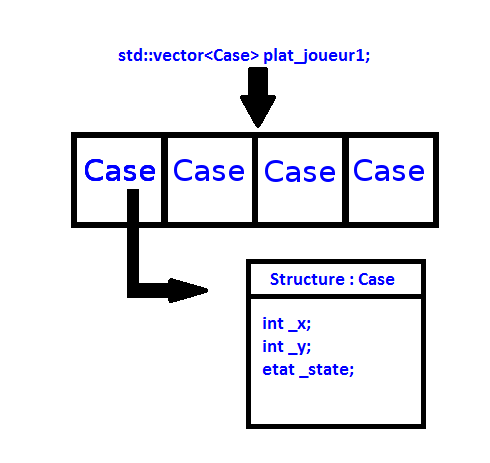
\includegraphics[width=5cm]{VectorCase.png} 
\end{center} 


Nous avons donc une case qui prend des coordonnées x,y afin de nous repérer dans le vecteur, ensuite nous avons créé une énumération "etat" qui prends les valeurs "VIDE, RATE, TOUCHE, BATEAU, COULE".  
Donc grâce à notre vecteur nous avons accès à la position de la case puis son état.
\newline
\\


Pareillement pour le bateau, nous avons ses coordonnées (x,y), sa longueur (2,3,4 ou 5), une direction (NORD, EST, OUEST , SUD) qui ont été définie dans un fichier qui contient les variables globales. Le nombre de fois que le bateau a été touché et un id.
Quand un bateau reçoit un tire on l'identifie grâce à son id, puis celui-ci incrémente la valeur du nombre de fois qu'il a été touché. Si la longueur du bateau est égale au nombre de fois qu'il a été touché, alors on supprime le bateau vecteur et change les cases correspondantes en "COULE".

\begin{center}
	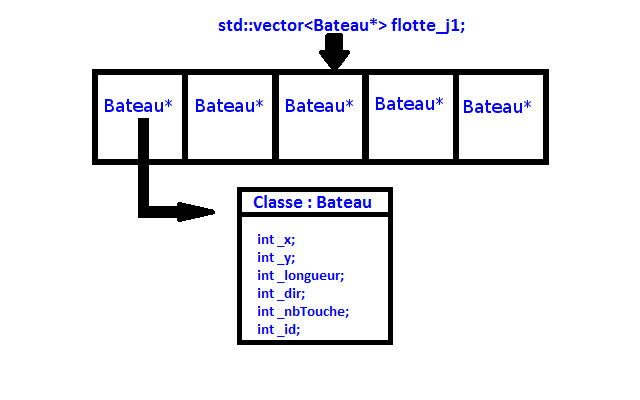
\includegraphics[width=7cm]{VectorBateau.png} 
\end{center} 



Nous avons également une classe Joueur qui nous permet de savoir si c'est le joueur 1 ou le joueur 2 qui joue le tour. Puis un type qui est égale soit à 0 (HUMAIN) soit à 1 (IA). 
\newline
\\

Grâce à ces éléments nous avons de quoi créer le plateau de jeu des joueurs, nous pouvons également créer et placer nos bateaux, ainsi que choisir le mode de jeu (IA vs IA ou Humain vs IA).
 

\subsection{Présentation }
Après compilation grâce au Makefile et que nous exécutons notre programme nous obtenons notre menu de jeu.

\begin{center}
	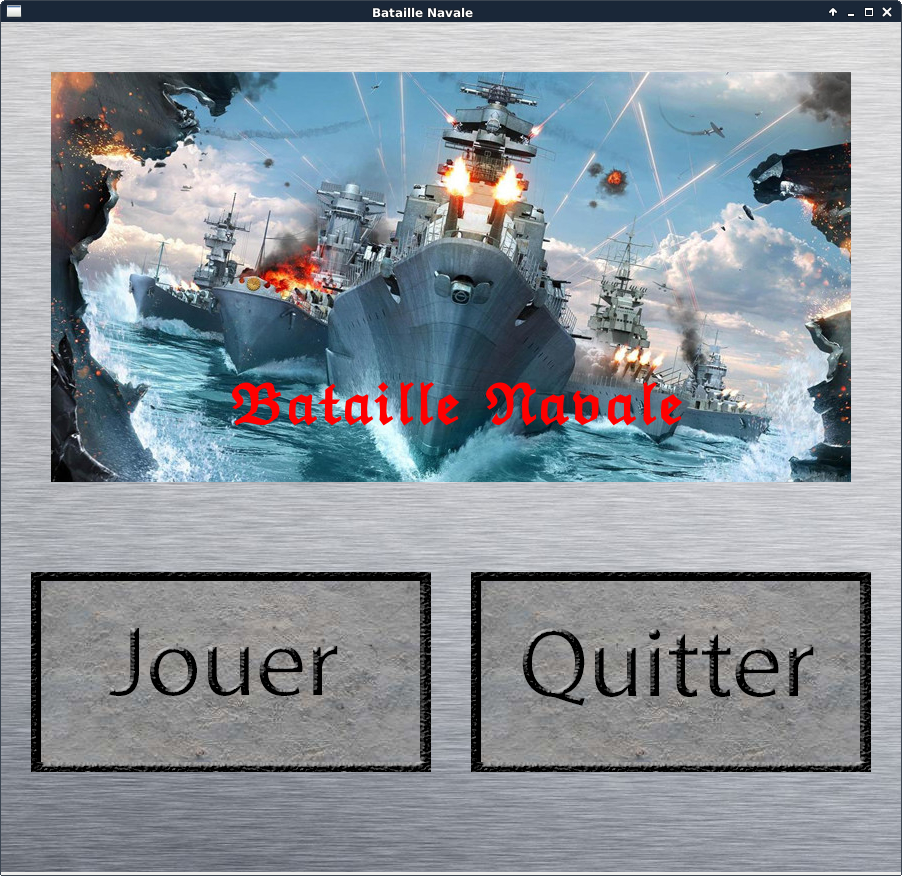
\includegraphics[width=7cm]{menuPrincipal.png} 
\end{center} 

Nous pouvons alors soit jouer une partie, soit quitter le jeu.

Si l'utilisateur choisit de jouer une partie alors il est redirigé vers d'autres menus :
\begin{itemize}
	\item Il devra alors choisir la difficulté de l'IA (Facile / Normal)
	\item Ensuite il choisit si le jeu est : Joueur vs IA ou IA vs IA
\end{itemize}

\begin{center}
	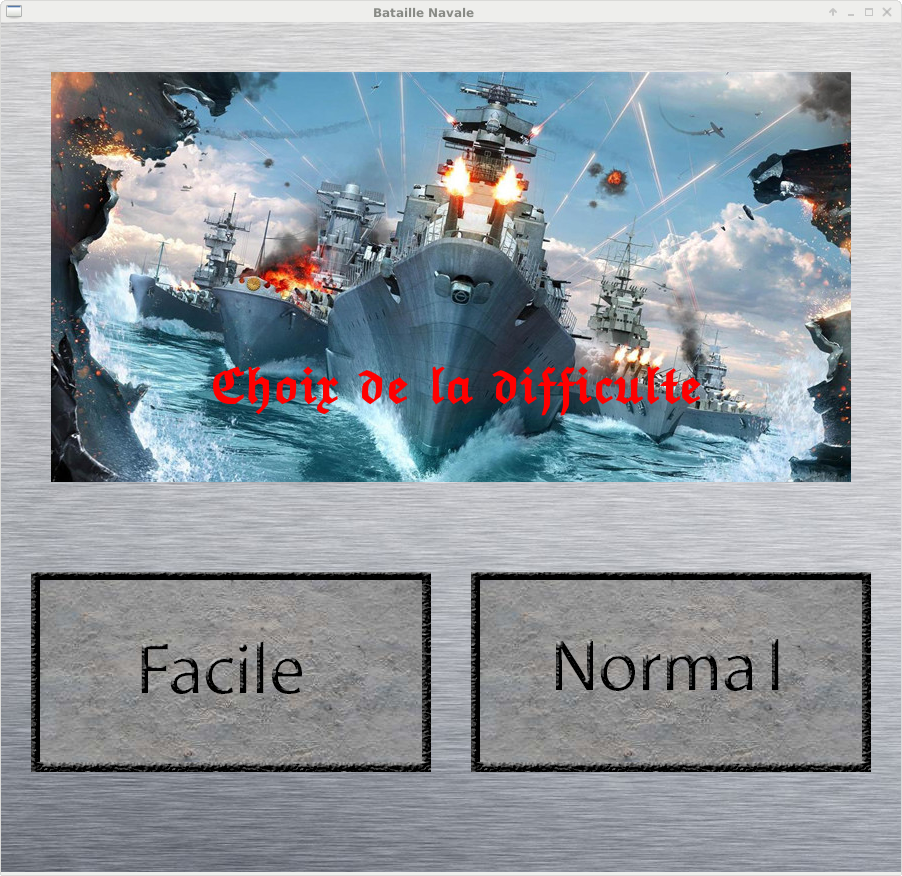
\includegraphics[width=7cm]{menuDifficulte.png} 
\end{center}

\begin{center}
	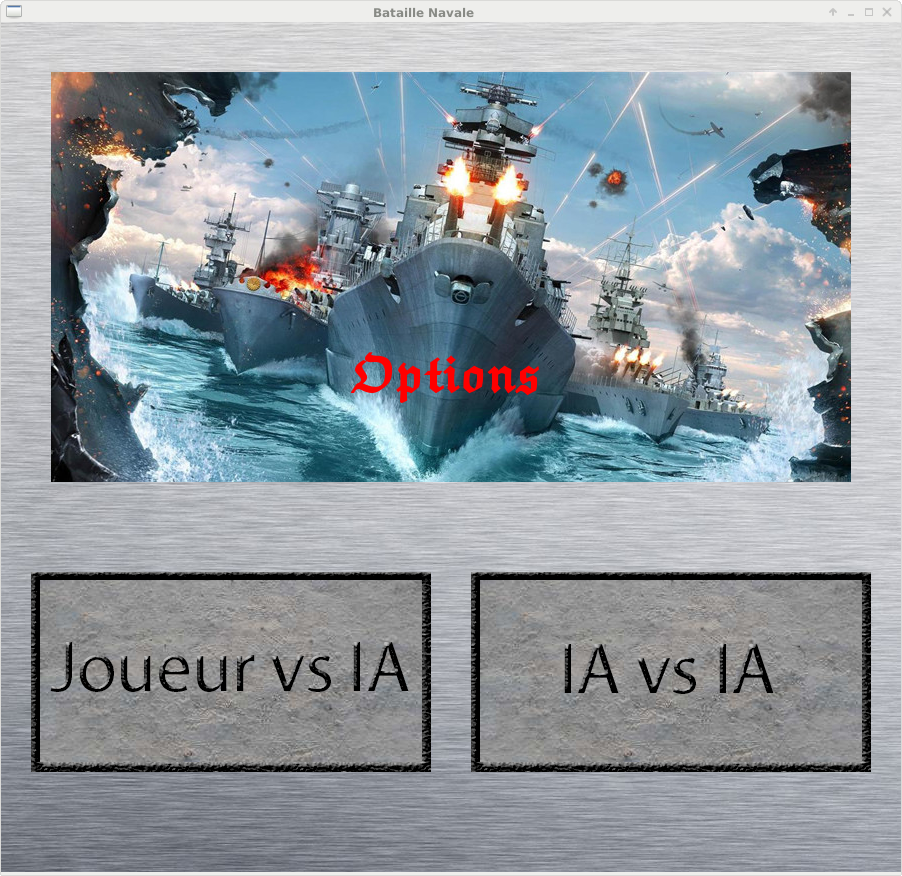
\includegraphics[width=7cm]{menuOptions.png} 
\end{center}

Une fois les modes de jeux choisit on arrive à l'écran de placement des bateaux :
\begin{itemize}
	\item Il peut choisir grâce aux flèches l'orientation du bateau qu'il veut placer
	\item Il peut cliquer sur la case souhaitée pour placer son bateau puis valider le placement de celui-ci
\end{itemize}

\begin{center}
	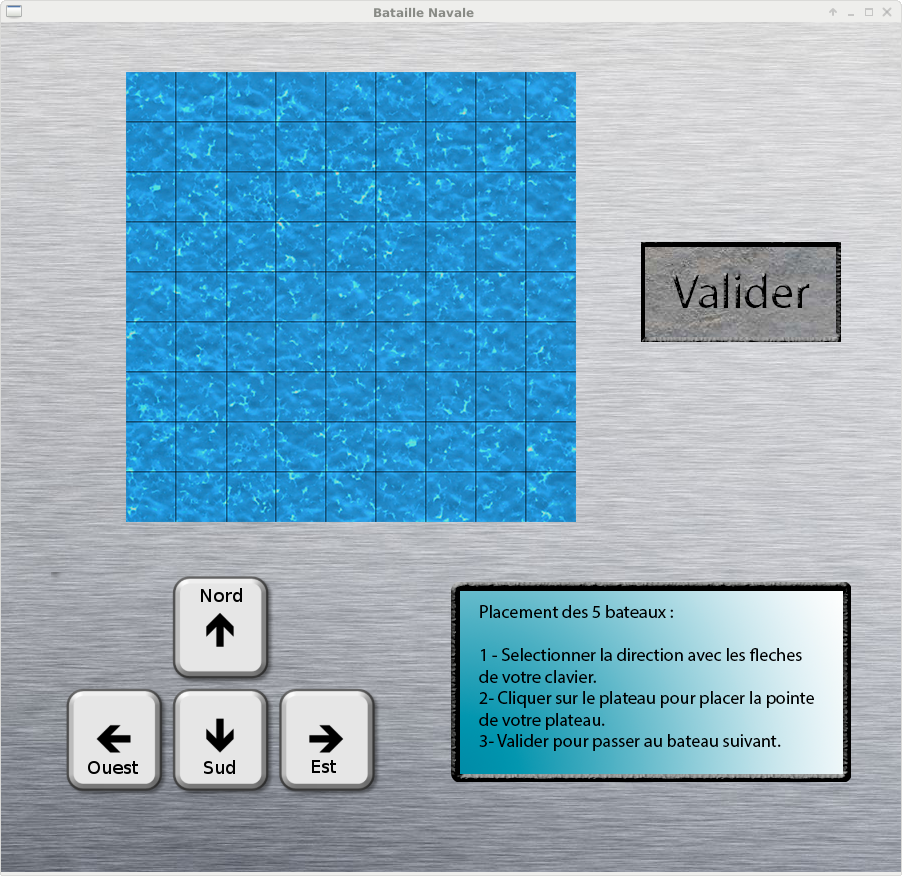
\includegraphics[width=7cm]{menuJouer.png} 
\end{center}

Une fois que le placement est terminé, la partie peut se lancer.
	

\begin{center}
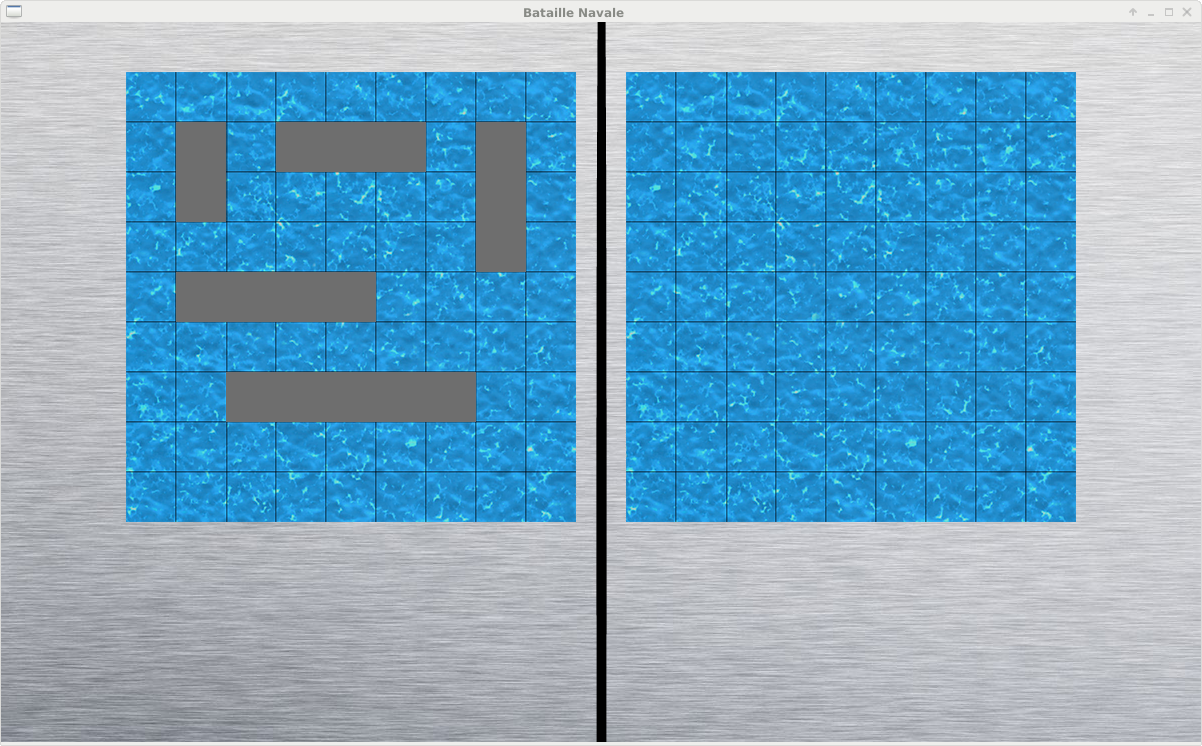
\includegraphics[width=9cm]{Jeu.png}
\end{center}



\paragraph{}
Enfin, comme convenu dans le cahier des charges, le logiciel fonctionne sur l'environnement Linux avec la bibliothèque SFML


\clearpage

%%%%%%%%%%%%%%%%%%%%%%%%%


\section{Bilan}


\subsection{Déroulement du projet}

Problèmes rencontrés et solutions adoptées :
\begin{itemize}

\item Pendant les 10 premiers jours du temps imparti pour réaliser notre projet, nous avons utilisé la librairie GTKMM pour réaliser notre interface graphique.Nous avons choisi cette librairie car c'est celle qui nous avions étudiée en cours, nous connaissions donc déjà les bases. Cependant, nous nous sommes aperçu que cette librairie était mal adaptée pour notre projet, notamment pour relier notre interface graphique a notre code. Nous avons donc opté pour une solution radicale : tout recommencer avec une nouvelle librairie qui nous semble mieux car écrite en langage C++, la librairie SFML.
\item Avec SFML, nous avons eu du mal a récupérer la grille où nous avions placé les bateaux pour la remettre sur la fenêtre suivante : celle du jeu. Pour résoudre ce problème, nous avons rassemblé menuPlateau.cpp et menuJouer.cpp. De cette manière, les deux fenêtres sont codées dans le même cpp et la grille de placement des bateaux est facilement récupérable.
\item Nous avions un problème de placement des bateaux étant donné qu'ils étaient placés dans un vecteur et pas un tableau. Nous avons dû trouver la formule pour placer la suite de notre bateau dans les bonnes cases
\item Pour l'IA, nous avons eu beaucoup de mal avec Min-Max, puisque la bataille navale est un jeu basé sur l'aléatoire
\newline
\\
\end{itemize}

Différences par rapport aux prévisions (conception, planification…) :
\begin{itemize}
	\item On utilise des rectangles pour symboliser les bateaux, et non pas des images de bateaux.
	\item Aucune implémentation de bruits/bruitages lors des tirs.
	\item Pas de gestion d'erreur lors du placement des bateaux.
	\item L'intelligence artificielle a demandé plus de temps que prévue, en particulier à cause de Min-Max
\end{itemize}	
	
\subsection{Réalisation des objectifs }

\begin{tabular}{| l | c |}
\hline
fonctionnalité & réalisation \\
\hline
\hline
Projet de base & complète \\
\hline
Interface graphique & partielle \\
\hline
IA & partielle \\
\hline
\end{tabular}

\paragraph{}
Pour l'interface graphique, il manque la vérification lors du placement des bateaux : si on place un bateau en dehors de la grille ou sur un autre bateau, on obtient une erreur de segmentation. De plus, lorsqu'on place les bateaux, il faut cliquer le plus légèrement possible sur valider, car si on reste appuyé trop longtemps, l'interface va détecter plusieurs cliques et certains bateaux pourraient ne pas être placés.
\newline
\\

A l'heure actuelle, il est impossible de jouer à notre jeu via l'interface graphique, car par manque de temps, nous n'avons pas entièrement relié le jeu console avec l'interface graphique.


Ce qui est fonctionnel dans l'interface graphique :
\begin{itemize}
	\item Le placement des bateaux pour le joueur
	\item Le choix de la difficulté
	\item Le choix du mode de jeu
	\newline
	\\
\end{itemize}

Ce qui n'est pas fonctionnel dans l'interface graphique :
\begin{itemize}
	\item Le placement des bateaux pour l'IA
	\item Jouer une partie
\end{itemize}

\paragraph{}
Pour L'IA, nous rencontrons un problème: L'IA ne va pas jusqu'au bout de la victoire

\subsection{Conclusion pour les projets futurs}

Ce qui a bien marché :
\begin{itemize}
	\item La cohésion de groupe
	\item La répartition des tâches
	\newline
	\\
\end{itemize}

Les erreurs à ne plus commettre :
\begin{itemize}
	\item Ne plus se précipiter sur une bibliothèque en début de projet sans réfléchir.
	\item Github : Ne pas faire le projet sur la branch master (comme nous avions fait les premiers jours), surtout si nous travaillons en plusieurs groupe
\end{itemize}



%%%%%%%%%%%%%%%%%%%%%%%%%

\label{myLastPage}

\end{document}

%%%%%%%%%%%%%%%%%%%%%%%%%

